\documentclass[man]{apa6}
\usepackage{lmodern}
\usepackage{amssymb,amsmath}
\usepackage{ifxetex,ifluatex}
\usepackage{fixltx2e} % provides \textsubscript
\ifnum 0\ifxetex 1\fi\ifluatex 1\fi=0 % if pdftex
  \usepackage[T1]{fontenc}
  \usepackage[utf8]{inputenc}
\else % if luatex or xelatex
  \ifxetex
    \usepackage{mathspec}
  \else
    \usepackage{fontspec}
  \fi
  \defaultfontfeatures{Ligatures=TeX,Scale=MatchLowercase}
\fi
% use upquote if available, for straight quotes in verbatim environments
\IfFileExists{upquote.sty}{\usepackage{upquote}}{}
% use microtype if available
\IfFileExists{microtype.sty}{%
\usepackage{microtype}
\UseMicrotypeSet[protrusion]{basicmath} % disable protrusion for tt fonts
}{}
\usepackage{hyperref}
\hypersetup{unicode=true,
            pdftitle={Replication of Experiment 2 from Nairne, Pandeirada, and Thompson (2008) `The Comparative Value of Survival Processing'},
            pdfauthor={Aira Contreras},
            pdfkeywords={Replication, Adaptive Memory, Survival, Graduate Class},
            pdfborder={0 0 0},
            breaklinks=true}
\urlstyle{same}  % don't use monospace font for urls
\usepackage{graphicx,grffile}
\makeatletter
\def\maxwidth{\ifdim\Gin@nat@width>\linewidth\linewidth\else\Gin@nat@width\fi}
\def\maxheight{\ifdim\Gin@nat@height>\textheight\textheight\else\Gin@nat@height\fi}
\makeatother
% Scale images if necessary, so that they will not overflow the page
% margins by default, and it is still possible to overwrite the defaults
% using explicit options in \includegraphics[width, height, ...]{}
\setkeys{Gin}{width=\maxwidth,height=\maxheight,keepaspectratio}
\IfFileExists{parskip.sty}{%
\usepackage{parskip}
}{% else
\setlength{\parindent}{0pt}
\setlength{\parskip}{6pt plus 2pt minus 1pt}
}
\setlength{\emergencystretch}{3em}  % prevent overfull lines
\providecommand{\tightlist}{%
  \setlength{\itemsep}{0pt}\setlength{\parskip}{0pt}}
\setcounter{secnumdepth}{0}
% Redefines (sub)paragraphs to behave more like sections
\ifx\paragraph\undefined\else
\let\oldparagraph\paragraph
\renewcommand{\paragraph}[1]{\oldparagraph{#1}\mbox{}}
\fi
\ifx\subparagraph\undefined\else
\let\oldsubparagraph\subparagraph
\renewcommand{\subparagraph}[1]{\oldsubparagraph{#1}\mbox{}}
\fi

%%% Use protect on footnotes to avoid problems with footnotes in titles
\let\rmarkdownfootnote\footnote%
\def\footnote{\protect\rmarkdownfootnote}


  \title{Replication of Experiment 2 from Nairne, Pandeirada, and Thompson (2008) `The Comparative Value of Survival Processing'}
    \author{Aira Contreras\textsuperscript{1}}
    \date{}
  
\shorttitle{Adaptive Memory}
\affiliation{
\vspace{0.5cm}
\textsuperscript{1} Brooklyn College of the City University of New York}
\keywords{Replication, Adaptive Memory, Survival, Graduate Class\newline\indent Word count: X}
\usepackage{csquotes}
\usepackage{upgreek}
\captionsetup{font=singlespacing,justification=justified}

\usepackage{longtable}
\usepackage{lscape}
\usepackage{multirow}
\usepackage{tabularx}
\usepackage[flushleft]{threeparttable}
\usepackage{threeparttablex}

\newenvironment{lltable}{\begin{landscape}\begin{center}\begin{ThreePartTable}}{\end{ThreePartTable}\end{center}\end{landscape}}

\makeatletter
\newcommand\LastLTentrywidth{1em}
\newlength\longtablewidth
\setlength{\longtablewidth}{1in}
\newcommand{\getlongtablewidth}{\begingroup \ifcsname LT@\roman{LT@tables}\endcsname \global\longtablewidth=0pt \renewcommand{\LT@entry}[2]{\global\advance\longtablewidth by ##2\relax\gdef\LastLTentrywidth{##2}}\@nameuse{LT@\roman{LT@tables}} \fi \endgroup}


\DeclareDelayedFloatFlavor{ThreePartTable}{table}
\DeclareDelayedFloatFlavor{lltable}{table}
\DeclareDelayedFloatFlavor*{longtable}{table}
\makeatletter
\renewcommand{\efloat@iwrite}[1]{\immediate\expandafter\protected@write\csname efloat@post#1\endcsname{}}
\makeatother

\authornote{This project has been done for Professor Crumps' Spring 2019 Special Topics in Experimental Psychology Pscy. 7709G.

Correspondence concerning this article should be addressed to Aira Contreras, Not Applicable. E-mail: \href{mailto:aira.contreras@gmail.com}{\nolinkurl{aira.contreras@gmail.com}}}

\abstract{
The experiments in the Nairne, Pandeirada, and Thompson (2008) paper test human memory systems in survival and non-survival conditions in an effort to determine if one yields measurably better recollection from participants. Participants were asked to rate words in conditions that produce excellent retention including conditions that had words related to pleasantness, imagery, and self reference. Previous experiments have suggested that participants show superior memory when words were related to survival conditions. The researchers suggest that this may be a result of fitness advantages accrued in the ancestral past. The goal of this exercise is to replicate one of the experiments presented in the paper and determine if the results were similar or even the same. The analysis will be done via the Rstudio software. I was able to {[}successfully/not successfully{]} replication the experiment.


}

\begin{document}
\maketitle

\hypertarget{methods}{%
\section{Methods}\label{methods}}

\hypertarget{participants}{%
\subsection{Participants}\label{participants}}

Twenty-four participants were recruited into the experiment. It is unclear what the demographics of these participants are, though it could be surmised that they may have been of the average undergraduate population (late teens, early twenties) because some were rewarded with partial credit to an introductory psychology course.

\hypertarget{apparatus}{%
\subsection{Apparatus}\label{apparatus}}

Two different experimental conditions were created: Survival and Vacation.These two conditions were further subdived into 4 experimental blocks. Participants were demonstrated each of the two conditions within the 4 blocks and tested individually in sessions that lasted approximatedly 30 minutes.

\hypertarget{materials-and-design}{%
\subsection{Materials and Design}\label{materials-and-design}}

In the study a set of 38 unrelated words (32 experimental words and 6 practice words) were created using the updated Battig and Montigue norms (Van Overschelde, Rawson, \& Dunlosky, 2004).Four blocks, each containing 8 words in random order, were created. Particpants all experienced the same random order. Participants were asked to rate 16 words with the survival scenario (S) and 16 words using the vacation scenario (V; see above criteria excluding Survival). The rating scale was from 1 (totally irrelevant) to 5(extremely relevant). Presentation of the words in 2 conditions (SVSV or VSVS) was followed by a retention invertval (digit recall task), and then an unexpected free recall was done to test memory.

\hypertarget{procedure}{%
\subsection{Procedure}\label{procedure}}

As described by the paper, participants were randomly assigned into one of the two experimental conditions upon arrival to the lab. Counterbalancing was taken into consideration. General instructions were provided instructing to rate words according to the particular scenarios. At the begining of each block, either the survival instructions appeared or the vacation instructions appeared; participants rated three practice words to ensure the two rating scenarios were understood. All blocks were presented, with the fourth block followed by a distractor task and then the surprise free-recall. For more detail on the instructions please read Experiment 1 procedure for Survival and Experiment 2 procedure for Vacation in Nairne et al. (2008).

\hypertarget{data-analysis}{%
\subsection{Data analysis}\label{data-analysis}}

A within-subjects analysis of variance (ANOVA) was conducted to analyze the data collected. Lecture from Dr.~Erin M. Buchanan used as learning tool to perform a within subjects ANOVA (Buchanan, 2018). Recommended R packages downloaded according to video instructions.

Original citation from papaja was also retained: \enquote{We used R (Version 3.5.2; R Core Team, 2018) and the R-packages \emph{devtools} (Version 2.0.1; Wickham et al., 2018), \emph{dplyr} (Version 0.8.0.1; Wickham et al., 2019), \emph{ez} (Version 4.4.0; Lawrence, 2016), \emph{ggplot2} (Version 3.1.0; Wickham, 2016), \emph{lattice} (Version 0.20.38; Sarkar, 2008), \emph{One-WayVid} (Buchanan, 2018), \emph{papaja} (Version 0.1.0.9842; Aust \& Barth, 2018), \emph{plyr} (Version 1.8.4; Wickham et al., 2019; Wickham, 2011), \emph{pwr} (Version 1.2.2; Champely, 2018), \emph{readxl} (Version 1.3.1; Wickham \& Bryan, 2019), \emph{reshape2} (Version 1.4.3; Wickham, 2007), \emph{Rmisc} (Version 1.5; Hope, 2013), \emph{schoRsch} (Version 1.5; Pfister \& Janczyk, 2018), and \emph{usethis} (Version 1.4.0; Wickham \& Bryan, 2018) for all our analyses.}

\newpage

\hypertarget{results}{%
\section{Results}\label{results}}

I was unsuccessful in the re-anlysis of the results, though I did learn about the different ways that data needs to be re-formatted in order to perform a within subject ANVOA analysis. The authors reported the following results F(1,23)=5.70, MSE=0.028, partial eta squared=.2. My results are F(1,24)=6.54,MSE=0.013, partial eta squared=.21, p=.017. I believe that the way the data was imported may have affected my results, as I ended up with 30 subjects as opposed to 24. The sort of data exclusions that the authors performed were not specified, so I had to do a lot of guessing that was not in line with what was intially performed by the authors. I also attempted to replicate a bar graph as they had and had more success in that round.

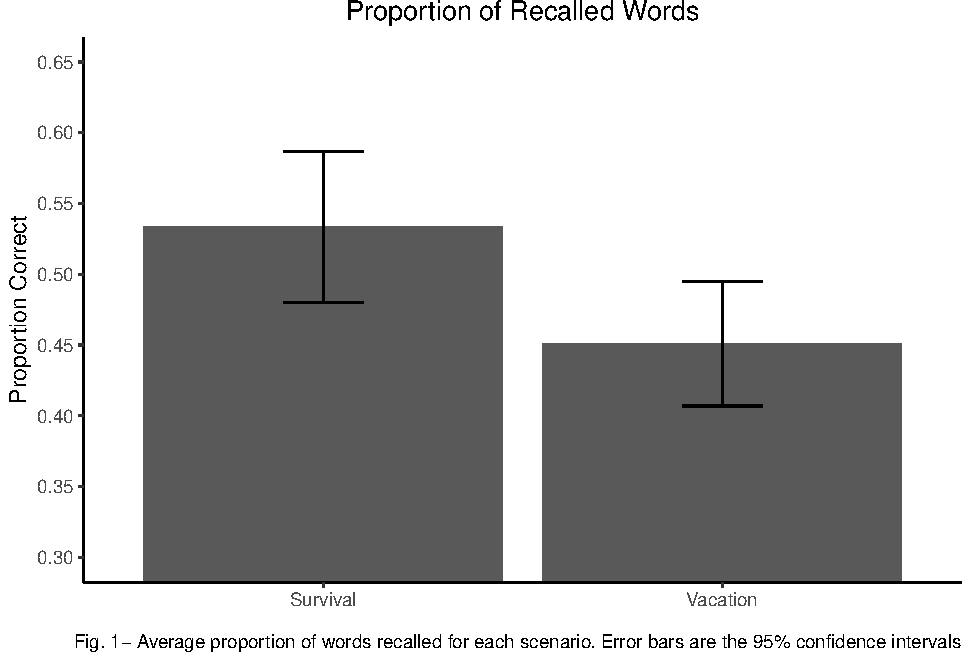
\includegraphics{Midterm_Project_files/figure-latex/unnamed-chunk-2-1.pdf}

\hypertarget{discussion}{%
\section{Discussion}\label{discussion}}

The authors were able to indicate that the Survival condition produced a greater proportion of correctly remembered words than the vacation group. Though I was not able to replicate this with confidence, I do not think it is that the effect is not there, but rather that I am not experienced enough in the data analysis portion of the project as required. Though I was not able to replicate the results, my results do come quite close with a p=.017, indicating statistical significance as my set alpha level was p=0.05.
\newpage

\hypertarget{references}{%
\section{References}\label{references}}

\begingroup
\setlength{\parindent}{-0.5in}
\setlength{\leftskip}{0.5in}

\hypertarget{refs}{}
\leavevmode\hypertarget{ref-R-papaja}{}%
Aust, F., \& Barth, M. (2018). \emph{papaja: Create APA manuscripts with R Markdown}. Retrieved from \url{https://github.com/crsh/papaja}

\leavevmode\hypertarget{ref-R-One-WayVid}{}%
Buchanan, D. E. M. (2018). \emph{R- one-way repeated measures anova example}. Unknown: Missouri State University. Retrieved from \url{https://www.youtube.com/watch?v=OeQqSZ6GJck}

\leavevmode\hypertarget{ref-R-pwr}{}%
Champely, S. (2018). \emph{Pwr: Basic functions for power analysis}. Retrieved from \url{https://github.com/heliosdrm/pwr}

\leavevmode\hypertarget{ref-R-Rmisc}{}%
Hope, R. M. (2013). \emph{Rmisc: Rmisc: Ryan miscellaneous}.

\leavevmode\hypertarget{ref-R-ez}{}%
Lawrence, M. A. (2016). \emph{Ez: Easy analysis and visualization of factorial experiments}. Retrieved from \url{http://github.com/mike-lawrence/ez}

\leavevmode\hypertarget{ref-nairne2008adaptive}{}%
Nairne, J. S., Pandeirada, J. N., \& Thompson, S. R. (2008). Adaptive memory: The comparative value of survival processing. \emph{Psychological Science}, \emph{19}(2), 176--180.

\leavevmode\hypertarget{ref-R-schoRsch}{}%
Pfister, R., \& Janczyk, M. (2018). \emph{SchoRsch: Tools for analyzing factorial experiments}. Retrieved from \url{http://www.tqmp.org/RegularArticles/vol12-2/p147/index.html}

\leavevmode\hypertarget{ref-R-base}{}%
R Core Team. (2018). \emph{R: A language and environment for statistical computing}. Vienna, Austria: R Foundation for Statistical Computing. Retrieved from \url{https://www.R-project.org/}

\leavevmode\hypertarget{ref-R-lattice}{}%
Sarkar, D. (2008). \emph{Lattice: Multivariate data visualization with r}. New York: Springer. Retrieved from \url{http://lmdvr.r-forge.r-project.org}

\leavevmode\hypertarget{ref-van2004category}{}%
Van Overschelde, J. P., Rawson, K. A., \& Dunlosky, J. (2004). Category norms: An updated and expanded version of the norms. \emph{Journal of Memory and Language}, \emph{50}(3), 289--335.

\leavevmode\hypertarget{ref-R-reshape2}{}%
Wickham, H. (2007). Reshaping data with the reshape package. \emph{Journal of Statistical Software}, \emph{21}(12), 1--20. Retrieved from \url{http://www.jstatsoft.org/v21/i12/}

\leavevmode\hypertarget{ref-R-plyr}{}%
Wickham, H. (2011). The split-apply-combine strategy for data analysis. \emph{Journal of Statistical Software}, \emph{40}(1), 1--29. Retrieved from \url{http://www.jstatsoft.org/v40/i01/}

\leavevmode\hypertarget{ref-R-ggplot2}{}%
Wickham, H. (2016). \emph{Ggplot2: Elegant graphics for data analysis}. Springer-Verlag New York. Retrieved from \url{http://ggplot2.org}

\leavevmode\hypertarget{ref-R-usethis}{}%
Wickham, H., \& Bryan, J. (2018). \emph{Usethis: Automate package and project setup}. Retrieved from \url{https://github.com/r-lib/usethis}

\leavevmode\hypertarget{ref-R-readxl}{}%
Wickham, H., \& Bryan, J. (2019). \emph{Readxl: Read excel files}.

\leavevmode\hypertarget{ref-R-dplyr}{}%
Wickham, H., François, R., Henry, L., \& Müller, K. (2019). \emph{Dplyr: A grammar of data manipulation}.

\leavevmode\hypertarget{ref-R-devtools}{}%
Wickham, H., Hester, J., \& Chang, W. (2018). \emph{Devtools: Tools to make developing r packages easier}. Retrieved from \url{https://github.com/r-lib/devtools}

\endgroup


\end{document}
